\documentclass[a4paper,10pt]{article}
\usepackage[utf8x]{inputenc}
\usepackage{amsmath}
\usepackage{amsfonts}
\usepackage{relsize}
\usepackage[smaller]{acronym}
\usepackage{graphicx}
\usepackage{subfigure}
\usepackage{cite}
\usepackage{url}
\usepackage{hyperref}
\usepackage{color}
\usepackage[version=3]{mhchem}
\usepackage{wrapfig}

\usepackage[left=2.5cm,right=2.5cm,top=2.5cm,bottom=2.5cm]{geometry}

\acrodef{WSN}{Wireless sensor network}
\acrodef{TEG}{Thermoelectric generator}
\acrodef{EH}{Energy harvesting}
\acrodef{PZT}{lead zirconate titanate}
\acrodef{RTG}{Radioisotope Thermoelectric Generator}
\acrodef{IBM}{IBM}

%opening
\title{Energy Harvesting}
\author{Author: Miha \v Can\v cula \\ Mentor: doc. dr. Du\v san Ponikvar}

\renewcommand{\vec}{\mathbf}
\renewcommand{\refname}{\section{Sources}}

\begin{document}

\begin{center}

\includegraphics[width=6cm]{./logo_fmf_uni-lj_sl}\\[0.5cm]
Oddelek za fiziko \\[2cm]
{ \large Seminar -- 1. letnik, II. stopnja } \\[1cm]
{ \huge \bf Energy Harvesting }\\[2cm]
{\large Author: Miha \v Can\v cula}\\[0.6cm]
{\large Mentor: doc. dr. Du\v san Ponikvar} \\[0.6cm]
{\large Ljubljana, januar 2012}
\end{center}
\vfill
\begin{abstract}

Technological developments in the recent years has allowed smaller and smaller electronic devices with very low power consumption. On the other hand, power generation methods are improving as well, increasing their efficiency and lowering costs. Now we are at the point where the two ends meet, as it becomes possible and economically justifiable for each device to have its own power source. The benefits of this are apparent: the possibility of delivering electricity to remote locations, next to nonexistant maintenance, and often just convenience. 

In this seminar, I will show where such devices are most commonly used and what power requirements they have, as well as present the three most popular methods for generating energy from the environment. With the low and irregular power output, proper power management and energy storing are important in ensuring the constant operation of the powered device, so I will focus on them as well. Finally, I will list some existing and succesful implementations of systems powered by harvested energy. 

\end{abstract}


\newpage
\tableofcontents

\newpage
\section{Introduction}

Small electronic devices are increasingly present everywhere around us. With their ubiquity and ever decreasing size and power consumption, connecting each of them to the power grid becomes impractical. 

The traditional solution is to use batteries, but they come with their own set of problems. Replacing them can be expensive, especially in hard-to-reach places. A much better option would be if the device had a power source of its own, removing its dependence on the power grid and drastically reducing the maintenance cost~\cite{Burgoine11}. 

The practice of drawing small amounts of electricity from the device's immediate surrounding is called \ac{EH}. 

\section{Use-cases}

\subsection{Sensors}

A very common use for energy harvesting systems are nodes in \acp{WSN}~\cite{teg-wsn-ieee,cap-wsn-ieee}. Such a network can contain a large number of independent nodes, so it would be difficult to connect each node to the power grid with wires. The sensors themselves usually consume very small amounts of power, so they are ideal applications for \acl{EH} methods. A block diagram of a generic sensor node can be seen in Figure~\ref{fig:block-sensor}. 

\begin{figure}[!h]
 \centering
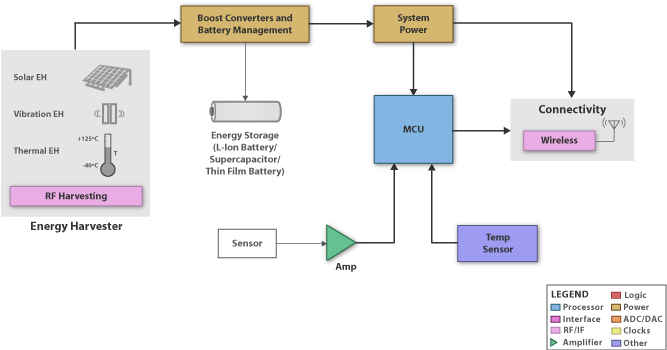
\includegraphics[width=.9\textwidth]{./Slike/EH-Block}
\caption{Block diagram of an \ac{EH}-powered wireless sensor node~\cite{ti:eh}}
\label{fig:block-sensor}
\end{figure}

The applications for \acp{WSN} include~\cite{wiki:eh}:
\begin{itemize}
  \item Weather stations
  \item Air and water pollution measuring
  \item Fire detection
  \item Industrial machine health monitoring
  \item Structural monitoring in buildings
  \item Intelligent buildings~\cite{cap-wsn-ieee}
\end{itemize}

Most of these applications require the nodes to be outside or in other areas where a direct connection to the grid would be difficult. On the other hand, they can still be close enough to the central node so they can transmit the measurements over a wireless connection with their own harvested power. 

Another important characteristic of sensor nodes is their power consumption profile. Often they will be idle for a long time (from minutes to days), and perform measurements in a relatively short time. The transmission of data can be even more infrequent, depending on whether the data has to be available immediately or not. In any case, sensor nodes consume very little current in the idle time period, with short bursts of consumption at regular intervals. An example of such consumption profile is in Figure~\ref{fig:wsn-consumption}. 

\begin{figure}[h]
\centering
 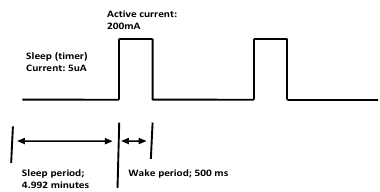
\includegraphics[width=250pt]{./Slike/wsn-current-profile}
 \caption{A plot of current consumption versus time for a wireless sensor node~\cite{cap-wsn-ieee}}
\label{fig:wsn-consumption}
\end{figure}

The average power consumption depends mostly on the duty cycle. If the measurement and especially the transmission of data  does not have to be continuous, but only happens in long intervals, the average consumption can be made very low. The consumption during the inactive time is often of the order of a few $\mu W$~\cite{Salerno10}. For example, electrical characteristic of an automatic radiator valve which take a measurement every hour are listed in Table~\ref{tab:zbarv}. This system draws an average power of 1 mW and would need its batteries changed at least once a year without any harvested energy~\cite{teg-wsn-ieee}. 

\begin{table}[h]
  \centering
  \begin{tabular}{|c|c|}
\hline
    Parameter & Value \\
\hline
Supply Voltage & 2.7 - 3.3V \\
Working current & 60 mA \\
Sleeping current & 10 $\mu$A \\
Working duration & 20 seconds/hour \\
Sleeping duration & 3579 seconds/hour \\
\hline
  \end{tabular}
\caption{Electrical characteristics of an automated radiator valve}
\label{tab:zbarv}
\end{table}

\subsection{Consumer electronics}

Many popular electronic devices, including TV remote controls, digital watches, portable music players and mobile phones, have power consumption low enough to be powered or at least assisted by \ac{EH}. Although their batteries can last a very long time, they can run out unexpectedly and cause a severe inconvenience. 

Solar cells on pocket calculators are very common and well-known, but so far their use has not spread to other electronic devices. There are, however, studies and working examples of remote controls for television and cars using a piezoelectric generator powered by the pressing force of our fingers, so this might change in the near future. 


\begin{figure}[h]
\centering
 \subfigure{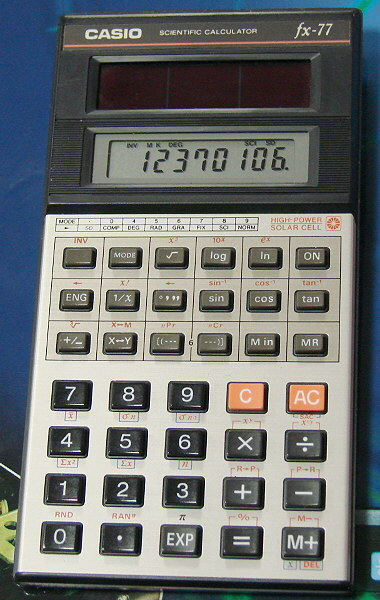
\includegraphics[height=180pt]{./Slike/casio-solar-calculator}}
 \subfigure{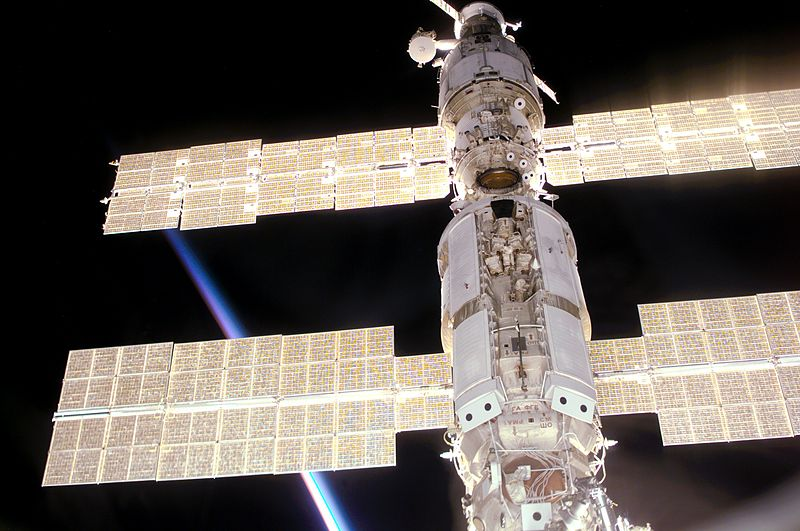
\includegraphics[height=180pt]{./Slike/ISS-solar}}
\caption{A solar-powered calculator by Casio (left) and the International Space Station with solar panels (right)~\cite{wiki:solar-cells}}
\end{figure}


\subsection{Spacecraft}

The impracticality of a grid connection or battery replacements is most evident in space. Satellites in orbit around Earth or travelling close to the Sun carry arrays of solar cells, harvesting energy from the Sun's radiation to power their systems. 

Deep-space probes, on the other hand, often fly too far from the Sun for solar energy to be a viable solution. Such probes are equipped with \acp{RTG} which convert heat from a slow radioactive decay to electricity. The farthest man-made object from Earth, Voyager 1, has been succesfully operating on \ac{RTG} power for nearly 35 years, and is projected to do so for at least 15 more. 

\section{Important properties}

When choosing the \ac{EH} method to use in a project, the most important factor is the available types of energy in the device's surroundings. These types will be explained in more detail in the following chapters. Additionally, most \ac{EH} devices are far from being an ideal power source. Therefore, we must carefully consider their electric properties before connecting them to a load. 

\subsection{Source resistance}

According to Th\'evenin's theorem, any combination of ideal voltage sources, current sources, and resistors with two terminals is electrically equivalent to a single voltage source in series with a single resistor. The resistor represents the source resistance or internal resistance of the power source. This simplified representation, while not completely accurate for real-world sources, serves as a good model for most power supplies and batteries~\cite{wiki:thevenin}. 

\begin{wrapfigure}{r}{.4\textwidth}
\centering
  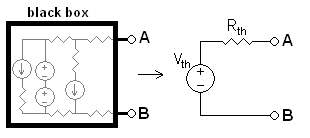
\includegraphics[width=150px]{./Slike/Thevenin_equivalent}
  \caption{A ``black box'' circuit and its Th\'evenin equivalent~\cite{wiki:thevenin}}
\label{fig:thevenin}
\end{wrapfigure}

A source with internal resistance $R$ and current $I$ wastes power equal to $I^2 R$, reducing the already limited power output, so we usually want power sources with a low source resistance. 

Source resistance is also important in power transfer. The most power is transferred when the source resistance is equal to the resistance of the load. This is often not the case with \ac{EH} sources where source resistance depends on environment conditions and can change with time. Fortunately, DC-DC converters exist which are able to increase or decrease both the voltage and resistance, providing matched resistances on both ends. 

It is important to note that all power sources mentioned here are direct current sources. Because of this, the imaginary component of the source impedance has no effect and use of the term resistance is justified. 

\subsection{Open-circuit voltage and short-circuit current}

Open-circuit voltage ($V_{oc}$) is the voltage between both terminals of the power source when no current is running through it. This is equivalent to loading it with an infinite-resistance load. This is the maximum voltage the source can produce; if a nonzero current is running, the source resistance will cause a voltage drop inside the source, resulting in a reduced output voltage. 

Short-circuit current ($I_{sc}$), on the other hand, specifies how much current the source is capable of generating under a load with zero resistance. In this case, the whole voltage drop happens inside the source, driving the output voltage to zero. 

In both of these extreme cases, the source produces no power. However, the characteristics are important because they are very easy to measure and compare. Sometimes these two pieces of information can be enough to make an informed choice of a power supply~\cite{Salerno10}. 

\subsection{$I(V)$ curve and power curve}

The current-voltage characteristic, also known as the $I(V)$ curve, shows how much current the generator can output at voltage $V$. Because all \ac{EH} sources have limited power, current will always drop if we put a load with a high resistance resistance on the source. Similarily, a low-resistance load will increase the voltage drop inside the source, causing the output voltage to decrease. 

A power curve is the relationship between the output power of the source and the load voltage. The electical power output is given by $P = V \cdot I$, so the current curve is simply the $I(V)$ curve multiplied by the voltage $V$. However, it is often the most important one as we wish to have the power source operate at its maximum power output. 

\subsection{Efficiency}

The ratio of electrical energy produced versus the solar, mechanical or thermal energy consumed is given by the {\em efficiency} of a power generator. Efficiencies of \ac{EH} sources vary greatly depending on their conversion method and size, but in general, they provide lower efficiencies than larger power sources. 

\section{Photovoltaic cells}

The best-known method of generating electricity from the environment on a small scale is using photovoltaic cells, also known as solar cells. In most environments, they provide the highest power output of all \ac{EH} devices. 

\subsection{Theory}

The solar cells work by using the photovoltaic effect to create electron-hole pairs in a two-layer semiconductor by exciting the electrons to the conduction band. Once in the conduction band, the electron moves to the n-doped side with lower potential without crossing the gap. The flow of electrons from one side of the cell to the other creates voltage between the two metal contacts~\cite{wiki:solar-cells}. A diagram of potential levels and the electron's path can be seen in Figure~\ref{fig:pv-band-diagram}. 

\begin{figure}[!h]
\centering
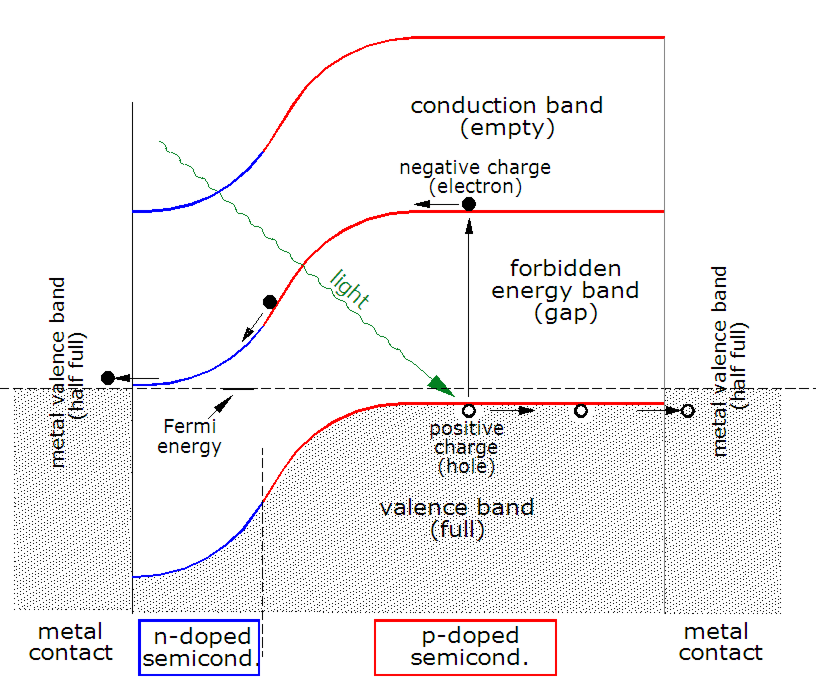
\includegraphics[width=0.7\textwidth]{./Slike/PV-band-diagram}
 \caption{Band diagram of the semiconductor inside a solar cell~\cite{wiki:solar-cells}}
\label{fig:pv-band-diagram}
\end{figure}

\subsection{Characteristics}

For photovoltaic cells, efficiency is the ratio between the electrical power output and the irradiation received by the cell and can reach up to 30\% in modern cells. However, it is possible to use mirrors or lenses to concentrate more sunlight onto the cell, effectively raising it efficiency up to 45\%. This is useful because the concentrating optics are usually cheaper than solar cells themselves. On the other hand, such concentrators often require a system for tracking the sun, resulting in a more complicated solution, and are better suited for large-scale operations than for energy harvesting devices. 

The maximum efficiency of photovoltaic cells is limited because a cell can only harvest photons with energy equal to the width of the semiconductor's bandgap. With the spectrum of sunlight, the highest possible efficiency is 37\%, also known as the Shockley–Queisser limit. This limitation can also be worked around by stacking several cells with different bandgaps in layers. This way, the theoretical limit can be raised up to 86\%~\cite{wiki:solar-cells}. 

Unlike other power sources, a photovoltaic cell can be modelled as an ideal current source connected in parallel with a diode. The open-circuit voltage is then equal to the diode's forward voltage, while the short-circuit current is the output of the model's source generator. A typical solar cell has a $V_{oc}$ of around half a volt. The short-circuit current and the maximum power output are both dependant on the light conditions and cell size. Because of the low voltage of a sigle photovoltaic cell, they are often connected in series. Alternatively, power can be drawn from a single larger cell with the help of a converter, at the cost of lower efficiency~\cite{Burgoine11}. 

The downside of solar generators is the constant changing of their power output, especially when used outdoors. An energy storage mechanism must be in place to provide power during the night and bad weather conditions. Even so, with variable weather conditions, the cell is not always operating with its peak efficiency. The shift in its optimal power point can be seen in Figure~\ref{fig:pv-power-curve}. It is possible to offset this by using a power management system that dynamically adjusts the cell voltage to find the maximum power point~\cite{solar-mppt-ieee}. 

\begin{figure}[h!]
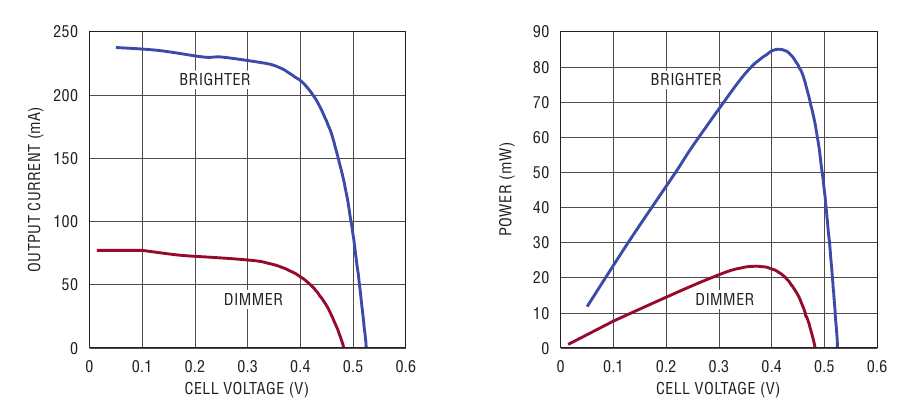
\includegraphics[width=\textwidth]{./Slike/PV-power-curve}
 \caption{Typical $I(V)$ and power curve of a 2x1 inch (13 cm$^2$) polycrystalline cell at two different irradiations~\cite{Burgoine11}}
\label{fig:pv-power-curve}
\end{figure}

\subsection{Light conditions}

Ambient light conditions are very important in determining the power output of photovoltaic cells. Besides only producing power during the daylight hours, solar cells are severely hindered by bad weather. In places with long periods of low light, such as rainy seasons or high lattitudes, large batteries are needed for energy storage. 

The situation is different if the cells are located inside a building. Indoors lighting is on average 400 times less intense than the irradiation by the Sun, resulting in correspondingly lower power outputs. However, the energy input is much more constant, especially the low-light periods are shorter and predictible. Despite the lower intensity, solar cells are useful even in indoors environments. Because most devices for indoor use can be made with power cords instead, the benefits of \ac{EH} are smaller there, but may still be significant with small and/or mobile devices. 

\section{\aclp{TEG}}


Another source of energy in the environment is a temperature gradient which can be converted into electricity using a \ac{TEG}. This method has become very popular in the recent years, mostly due to its reliability and lower cost than photovoltaics. Using the Seebeck effect, it is possible to convert the difference in temperatures into electricity.  The Seebeck effect is the converse of the better-known Peltier effect, so the same elements can be used for either thermoelectric cooling or power generation. Due to their simple design and the possibility to re-use existing Peltier coolers, \acp{TEG} can be much cheaper than other \ac{EH} devices. 

\subsection{Theory}

\acp{TEG} are typically made from a series of \textit{thermocouples}, pairs of n-doped and p-doped semiconductor pellets, sandwiched between two ceramic plates~\cite{Salerno10}. A schematic of their design can be seen in Figure~\ref{fig:teg-schematic}. 

\begin{figure}[h]
\subfigure{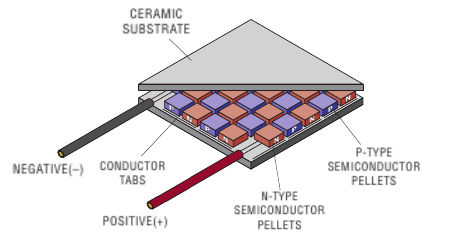
\includegraphics[height=100pt]{./Slike/TEG-shema}}
\subfigure{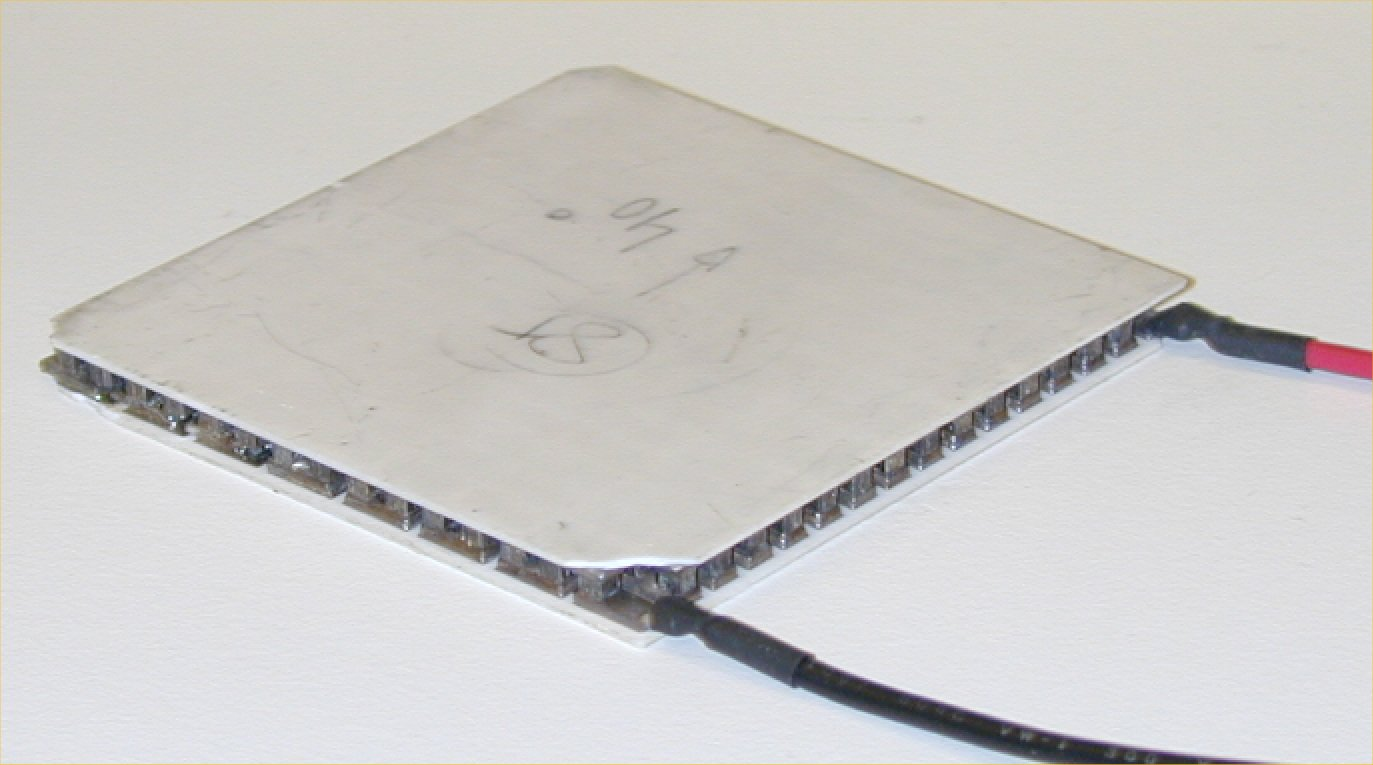
\includegraphics[height=100pt]{./Slike/TEG-slika}}
\caption{A schematic (left) and a photo (right) of a \ac{TEG} element~\cite{Salerno10,wiki:teg}}
\label{fig:teg-schematic}
\end{figure}


\begin{wrapfigure}{l}{.33\textwidth}
\centering
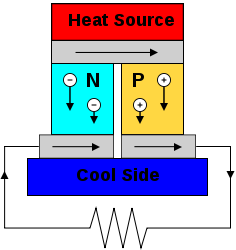
\includegraphics[height=135pt]{./Slike/TEG-couple}
 \caption{Detailed view of a single thermocouple~\cite{wiki:thermo}}
\label{fig:teg-couple}
\end{wrapfigure}

Figure~\ref{fig:teg-couple} shows a details view of a single thermocouple. Charge carriers on the hotter side move faster due to their higher thermal energy, so they diffuse towards the cold side. Bucause of the asymmetric diffusion, charge builds up on the colder side with the same sign as the charge carries in that semiconductor. By placing two opposite semiconductors side-by-side, we obtain a voltage between the electric leads~\cite{wiki:thermo}. 


The voltage is directly proportional to the temperature difference between the two sides. 

\begin{align}
 V &= -S \Delta T
\label{eq:seebeck}
\end{align}

Here $S$ is the Seebeck coefficient and is equal to the entropy per charge carrier of the material. Standard thermocouples made from a pair of metals have Seebeck coefficients of up to 100 $\mu$V/K, while semiconductors can reach values of almost 2000 $\mu$V/K~\cite{wiki:thermo,ec:seebeck}. 

\subsection{Characteristics}

Both the output voltage and the source resistance are directly proportional to the number of couples in the series, so it is important to use the right size of the generator to ensure a high enough voltage while still keeping the resistance low~\cite{Salerno10}. Since \acp{TEG} are heat engines, their efficiency is litimed by the Carnot efficiency $\eta = \Delta T / T_H$ and depends on the temperatures at both sides. In practice, it is even lower than that of other heat engines, only reaching a few percent~\cite{teg-curve,wiki:teg}. 

Characteristics of \texttt{TEC1-12709}, a common thermoelectric element which costs \$7.25, are given in Table~\ref{tab:teg-radiator}. Mounted on a radiator with temperature 30 K higher than that of the surrounding air, four such generators stacked in layers are capable of producing a maximum of 60 mW at 700 mV~\cite{teg-wsn-ieee}. 

\begin{table}[h]
  \centering
  \begin{tabular}{|c|c|}
\hline
    Parameter & Value \\
\hline
Dimensions & 30 x 34 x 3.2 mm \\
Maximum $\Delta T$ & 77 K \\
Number of couples & 127 \\
Device resistance & 3.78 $\Omega$ \\
\hline
  \end{tabular}
\caption{Physical properties of a \ac{TEG}}
\label{tab:teg-radiator}
\end{table}

At a constant temperature difference, \acp{TEG} have a linear $V(I)$ curve, such as the one in Figure~\ref{fig:teg-curve}. The power curve is a parabola, with the maximum power point at exactly half the open-circuit voltage. 

\begin{figure}[h]
\centering
 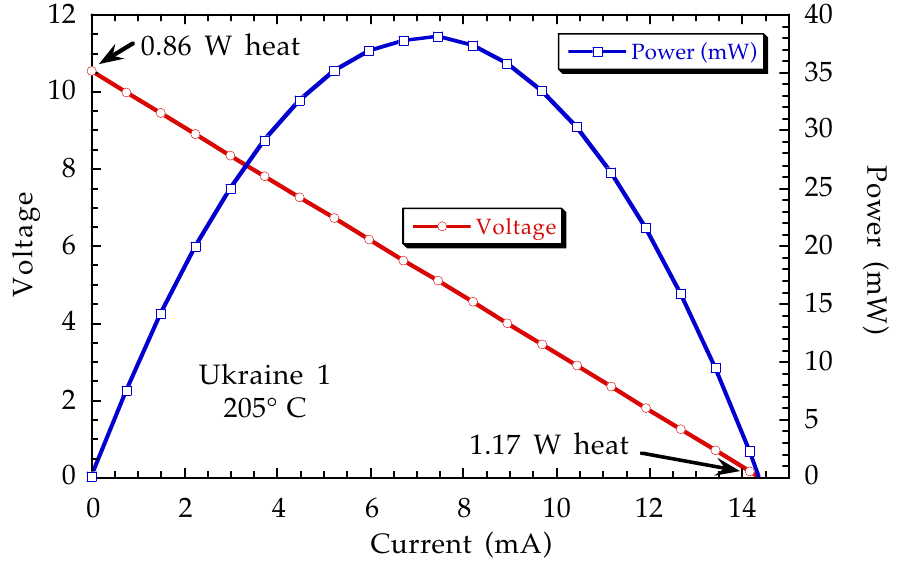
\includegraphics[height=150pt]{./Slike/TEG-curve}
\caption{$V(I)$ and power curve of a \ac{TEG}~\cite{teg-curve}}
\label{fig:teg-curve}
\end{figure}

\section{Piezoelectric generators}

The third most common form of \ac{EH} is generating power from the energy of motion. Vibrations are present especially in the vicinity of working machinery, but energy can also be produced from human activities, such as walking~\cite{piezo-shoe-ieee}. 

\subsection{Theory}

Certain crystalline materials with asymmetric unit cells polarize themselves when an external force is applied. This phenomenon is called the Piezoelectric effect. The best-known material to exhibit piezoelectric behavior is \ac{PZT}, a ceramic with the formula \ce{Pb[Zr_xTi_{1-x}]O3}, $0\leq x \leq 1$.

Like the thermoelectric effect, the piezoelectric effect also has a direct converse, where a voltage applied to the material causes it to deform. Because of this, the same elements can be used as actuators, capable of very precise positioning due to the high voltages required for small mechanical deformations. 

\begin{figure}[!h]
  \centering

\subfigure{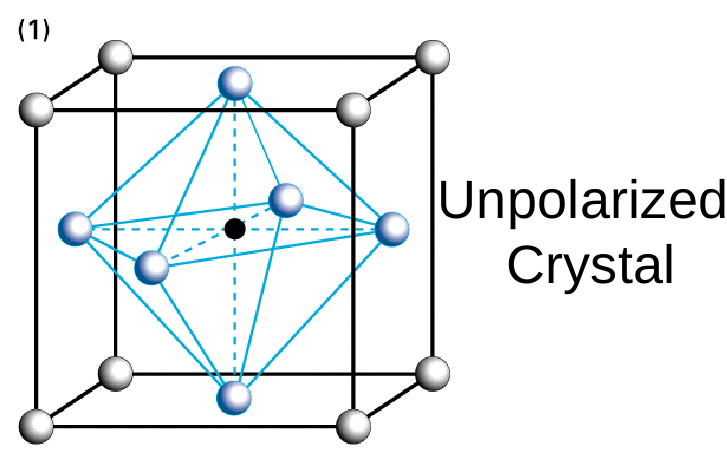
\includegraphics[width=150pt]{./Slike/Piezo-theory-normal}}\hspace{1cm}
\subfigure{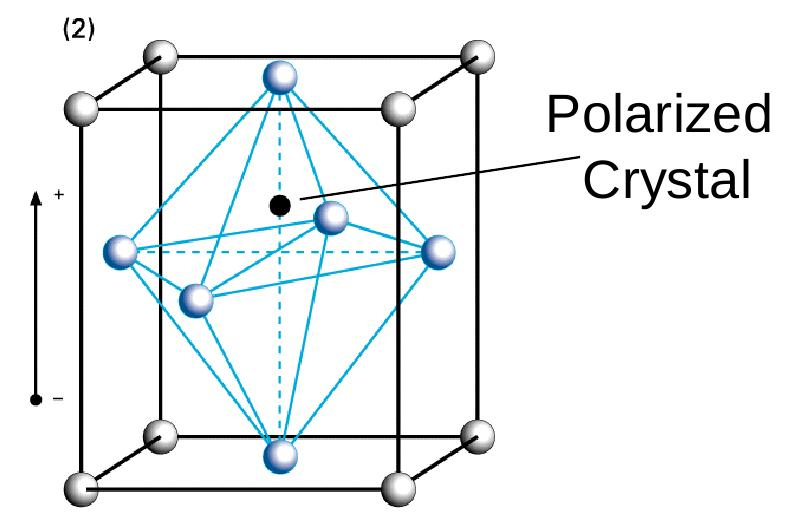
\includegraphics[width=150pt]{./Slike/Piezo-theory-polarized}}
\subfigure{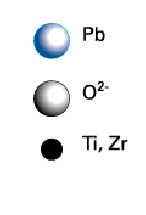
\includegraphics[width=40pt]{./Slike/Piezo-theory-legend}}
\caption{The change in charge distribution when a mechanical stress is applied to the crystal~\cite{cottone}}
\label{fig:piezo-theory}
\end{figure}

External pressure causes the ions in the lattice to rearrange. Due to their asymmetry, titanium and zirconium ions in the centre of every unit cell have a preferred direction of movement. A simplified representation of positions of ions in a single unit cell is shown in Figure~\ref{fig:piezo-theory}. Because the crystal is periodic, each unit cell polarizes in the same direction, causing an observable crystal-wide polarization~\cite{cottone}. 

In piezoelectric materials, the dielectric response $D = \varepsilon E$ and Hooke's law $S = sT$ are coupled~\cite{wiki:piezo}. 

\begin{align}
 \vec S &= s \vec T + d^t \vec E \\
 \vec D &= d \vec T + \varepsilon \vec E
\end{align}

Strain $\vec S$ and stress $\vec T$ are rank-2 tensors, but because they are always symmetric, they have only six free parameters and can be written as vectors with 6 components. Compliance $s$, permitivity $\varepsilon$ and piezoelectric matrix $d$ can now be written as rank-2 tensors. The first equation describes the converse piezoelectric effect (mechanic deformation under applied voltage) while the second describes the direct piezoelectric effect (polarization under applied stress). The polarization causes a difference in electric potential between the two sides of the piezoelectric, which can drive a current through a connected load. 

The values of $d$ are different for every material. For tetragonal and hexagonal crystals, only five out of 15 coefficients in the matrix are nonzero~\cite{wiki:piezo}. 

\subsection{Characteristics}

\begin{wrapfigure}{r}{.47\textwidth}
\centering
  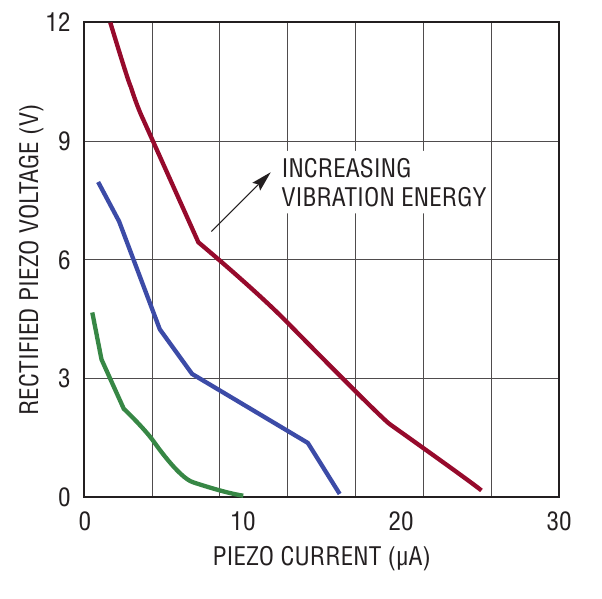
\includegraphics[width=0.45\textwidth]{./Slike/Piezo-UI}
\caption{Typical piezoelectric load lines~\cite{LT-Piezo}}
\label{fig:piezo-load}
\end{wrapfigure}

Unlike other \ac{EH} methods, piezoelectric elements often produce relatively high voltages, so a converter is needed to decrease the voltage. Both open-circuit voltage and short-circuit current increase with the available vibration energy~\cite{LT-Piezo}. Figure~\ref{fig:piezo-load} shows load lines for Piezo Systems \texttt{T220-A4-503X} with a wholesale price of \$70 per piece. We can observe that the lines are close to hyperbolas, so power output does not depend on the voltage applied, only on the vibration energy present. This particular element can function both as an energy harvester or an actuator and is rated for voltages up to $\pm$180 V. In typical vibration energy harvesting applications, the output voltage is much lower, but still high enough to require a specialized power supply. 

Using a smaller device, researchers were able to produce an average power of over 8 mW from a \ac{PZT}-based piezoelectric mounted inside a shoe. This was enough to continuously power a short range radio frequency emitter~\cite{piezo-shoe-ieee}. 

% Ne vem ce je to fajn vkljucit, je uporabno ampak staro (2000)
% According to research by Volvo Car Company, a piezo-element with dimensions of 67 x 25 x 1.45 mm requires the user to press a button with a force of 10 N to generate enough energy to send a signal to the car. 

\section{Power management}

As mentioned above, electrical power from \ac{EH} generators can be very sporadic, and so can be the required load. Therefore, additional electronics are require to turn the energy source into a useful power supply. 

\subsection{Voltage converters}

The first step is to ensure the maximum power transfer between the source and load. Differences in output voltage and resistance force us to use DC-DC converters. These converters can reach efficiencies of over 95\%, so they do not cause an excessive power loss. In changing conditions it is often necessary to dynamically adjust the converter to ensure the energy harvester is operating at its maximum power point~\cite{solar-mppt-ieee}. 

Depending on the output voltage of the power source, either step-up or step-down converters are used. Both are examples of switch-mode power supplies and function in a similar way, with an inductor for temporarily storing energy and two switches (a transistor and a diode) that control the inductor. A schematic of their design is shown in Figure~\ref{fig:converters}, however in most cases a capacitor is added in parallel with the load to reduce output voltage ripple~\cite{wiki:dcdc}. 

\begin{figure}[h!]
\centering
  \subfigure{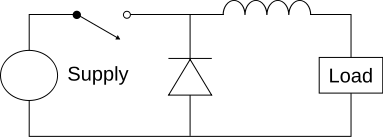
\includegraphics[height=72pt]{./Slike/Buck}}
  \subfigure{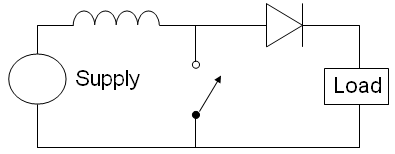
\includegraphics[height=80pt]{./Slike/Boost}}
\caption{Circuit diagrams of a step-down (left) and a step-up (right) DC converters. In both cases, the transistor is shown as an on-off switch~\cite{wiki:dcdc}.}
\label{fig:converters}
\end{figure}

The transistor periodically changes its state at a rate of 300kHz to 10MHz. In the continuous operation mode, when the inductor is never completely discharged, the voltage gain is only affected by the part of the time the transistor is in the ``on'' state, also known as the duty cycle $D$. The duty cycle is always between 0 and 1 and can be controlled, allowing the output voltage to be modified at will. The output voltage of a step-down converter can be expressed as

\begin{align}
  V_o &= V_i \cdot D \\
\intertext{while the equivalent expression for a step-up converter is}
  V_o &= V_i \cdot \frac{1}{1-D}
\end{align}


\subsection{Storage element chargers}

A major part of the power management system is the energy storage mechanism, responsible for the storage and retrieval of energy in a separate container. Due to the properties of the storage element, it is also responsible for limiting the current flow into the container to prevent overcharging. 

\subsection{Price}

Voltage and resistance converters for different energy sources, such as those made by Linear Technology and Texas Instruments, are available in bulk at \$1-\$4 per piece. Battery charge controllers are also widely available at low prices, around \$2 per piece. In total, the cost of the power management system is only a small part of the total cost of the power source, the majority being the energy harvester itself~\cite{lt:cenik, ti:eh}. 

\section{Energy storage}

The choice of the energy storage method depends on the application. For electronic devices such as phones or calculators, the most important characteristics are energy density and long life. On the other hand, wireless sensors require short bursts of power, calling for a storage element with high power density~\cite{cap-wsn-ieee}. Depending on the power source, the stored energy may have to power the device for long periods, favoring a storage element with a low self-discharge rate. 

In most cases, harvested energy is stored either in rechargeable batteries or ultracapacitors. Rechargeable batteries, while widely used, suffer from degradation over a large number of charge-discharge cycles, limiting their useful life. Ultracapacitors, also known as supercapacitors or Electric double-layer capacitors, are the newer technology, and are used where higher power density (as opposed to energy density) is required. Unlike conventional capacitors with two metallic plates and an insulator between them, ultracapacitors are composed of two layers of a single material with a very thin separator. The lack of a wide insulator permits a larger plate surface area in a given volume, but also limits their maximum voltage. 

\begin{figure}[h]
  \centering
  \includegraphics[width=.8\textwidth]{./Slike/Supercapacitor_diagram}
  \caption{Comparison of construction diagrams of three capacitors. Left: ``normal'' capacitor, middle: electrolytic, right: electric double-layer capacitor~\cite{wiki:edlc}}
  \label{fig:edlc-diagram}
\end{figure}

En example of such a system is a wireless sensor node with its short spike of power consumption during transmission of data. In cases where a single storage method cannot cover the needs of the powered device, a combination of a battery for long-term storage and an ultracapacitors for higher power output can also be used. 

An important difference in the electrical characteristics of the two types of storage elements is their internal resistance, which is much lower in ultracapacitors. The lower resistance allows for higher charge and discharge rates, but it also causes higher leakage currents. Other advantages of ultracapacitors include long life with no danger of overcharging or over-discharging, while their main disadvantages are lower energy density and high self-discharge rate~\cite{wiki:edlc}. 

\begin{figure}[!h]
\centering
\def\svgwidth{0.8\textwidth}
 \input{./Slike/Supercapacitors_chart.pdf_tex}
\caption{Comparison of energy storage options~\cite{wiki:edlc}}
\label{fig:storage-chart}
\end{figure}

Energy storage methods other than batteries and ultracapacitors are not widely used in energy harvesting. Fuel cells could be used in place of batteries, due to their high energy density and long life, but they are more complex and difficult to make in small sizes. They also require an external fuel source, negating the benefit of reduced size required to store the same amount of energy. Instead, they can used as an alternative to \ac{EH} as they don't need frequent refueling. Conventional capacitors, on the other hand, have very low energy densities and offer virtually no advantage over ultracapacitors. 

\section{Successful implementations}

\subsection{Building automation}

The EnOcean Alliance is a consortium of companies providing a building automation system with an open, interoperable standard for energy harvesting~\cite{enocean}. Its members offer wireless sensors, switches and controllers, capable of managing a building's lighting, heat, ventilation and air conditioning systems. Wireless communication is done in the 315Mhz and 868MHz bands, thus requiring less power than 2,4GHz used by the \texttt{IEEE 802.11} standards, traditionally used for wireless computer networks. An example wireless network with \ac{EH}-powered sensors and grid-connected central nodes and routers is in Figure~\ref{fig:enocean-shema}. 

\begin{figure}[h]
\centering
 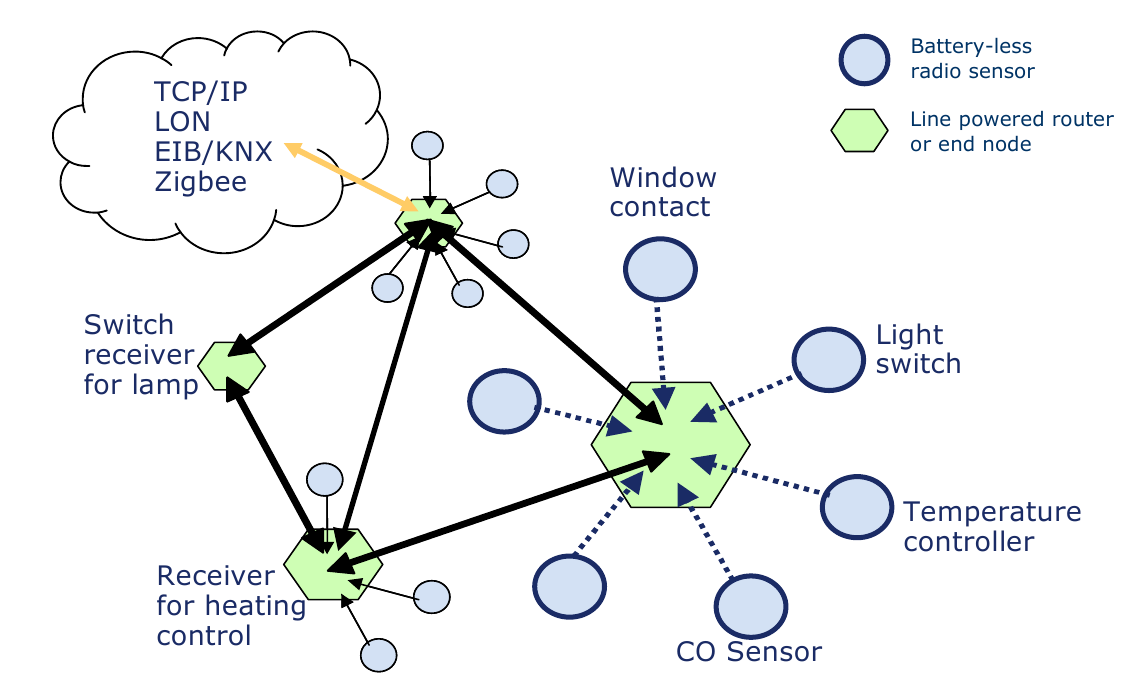
\includegraphics[width=0.9\textwidth]{./Slike/EnOcean-shema}
\caption{A wireless sensor network based on the EnOcean standard~\cite{enocean}}
\label{fig:enocean-shema}
\end{figure}

A competing group of companies constitute the ZigBee Alliance. Aside from building automation, they also offer health care and remote control applications. However, they have only recently began adopting \ac{EH}, with the first batteryless wireless switch presented by Schneider Electric in 2009~\cite{schneider-zb}. As we can see in Figure~\ref{fig:enocean-shema}, the two standards are compatible and can be linked via a gateway device. 

\newpage
\subsection{Phone and laptop chargers}

Several companies offer solar-powered chargers for phone and laptop batteries. In these cases, the goal is often not to power the devices solely through \ac{EH}, but mainly to extend battery life. 

A typical modern laptop computer under light load consumes an average power of around 20 watts. This is far beyond the range of small energy harvesting solutions, so the solar cells have to be very large, making them both more expensive and less portable. Solar laptop charges, powerful enough to provide at least 10 watts in optimal conditions, thus require almost half a square meter of surface area and can cost over \$500. However, smaller and cheaper power sources can still provide a significant increase in battery life, especially for smaller, less power-consuming laptops~\cite{news:laptop-chargers}. 

Mobile phones, on the other hand, require much less power. A phone spends most of the time in a sleeping state, in which it consumes less than 100 milliwatts. Hence the chargers can be the size of the phone itself and cost around \$30. With their small size, they cause no additional burden when being carried around, proving true energy harvesting devices~\cite{mysolarphonecharger}. 


\section{Conclusion}

\acf{EH} is becoming increasingly viable as a power source for small electronic devices. Because of their remote location or simply due to their small size and large count, it may become impractical or even impossible to connect such devices to the power grid or to supply them with batteries. Hence, an included small power source can drastically simplify the device installation and reduce its maintenance costs. \acs{IBM}, one of the largest technology companies in the world, predicts energy from walking and other unconventional sources will become widespread in the next five years~\cite{ibm:5in5}. 

We have seen three different methods for drawing power from the device surrounding, provided we have a source of light, heat or motion. The choice of a suitable method obviously depends on the device's power requirements and the environment in which it is meant to be used. There are other possible approaches, but these three are the most popular at this time. 

Because the energy source might not be present at all times, as is the case with photovoltaic placed outdoors, we also need to store the harvested energy. In this field, ultracapacitors are seeing rapid development and have become an alternative to more traditional batteries. Many wireless devices have a short duty cycle, during which the higher power output of capacitors is an important advantage, while their average power consumption is still very low. 

\newpage

\bibliography{harvesting}
\bibliographystyle{zumer} 

\end{document}
